% !TEX root = ../main.tex
\chapter{Supplementary Materials for \texorpdfstring{Chapter~\ref{ch:roil}}{Chapter 3}}\label{app:roil}

% ---- ported from the appendix of github.com/GersiD/ChebyshevROIL paper/RIRL_NHT.tex ----
\section{Proofs} % of \cref{sec:basic-formulation}}
\label{sec:appendix_proofs}
\begin{lemma}\label{prop:convexity_of_Upsilon}
The set $\Upsilon$ is non-empty, convex, compact, and polyhedral.
\end{lemma}
\begin{proof}
The set is non-empty because $u_{\mathrm{e}}\opt  \in \Upsilon$. It is convex and polyhedral from its construction and is compact because it is bounded ($1\tr u \le  \nicefrac{1}{1-\gamma}$) and closed.  
% Since $\mathcal{U}$ is the set of feasible solutions to the dual LP formulation~\cite[Eq.~(6.9.2)]{Puterman1994} it is well known to be polyhedral and convex. To show that the set $\mathcal{U}$ is compact, we need to show that it is bounded. This is true since, $u \in \mathcal{U}$ satisfies $u \ge 0$ by construction, and it is easy to verify that $1\tr u = \frac{1}{1-\gamma}$. Then, the set $\Upsilon$ is an intersection of half-spaces with $\mathcal{U}$ a closed convex set. Any union of closed half-spaces is convex and closed~\cite[eq.~(2.2.1)]{boyd_convex_optimization}.
\end{proof}

\lemmaOccupancyExistance*
\begin{proof}
We prove the two implications individually.

\emph{Case 1:} Prove $u \in \Upsilon   \quad \Rightarrow \quad  \exists
        \pi \in \Pi_{\mathrm{R}}(\mathcal{D}), \, u = u^{\pi}$,

Given a $u \in \Upsilon$, we have that $u^{\pi_{u}} = u$ since $u\in \mathcal{U}$ and $p_0 > 0$. Recall that $p_0 >0 $ guarantees that
\[
  \sum_{a\in \mathcal{A}} u(s,a) \ge  p_0 > 0, \quad \forall s\in \mathcal{S}.
\]
We now show that $\pi^u \in \Pi_{\mathrm{R}}(\mathcal{D})$. The constraint on $u\in \Upsilon$ combined with $u > 0$ implies that for each $(\cdot , s, \cdot ) \in \mathcal{D}$:
\begin{alignat*}{2}
  && \sum_{a\in \mathcal{A} : a \neq \pi_{\mathrm{e}}(s)} u(s,a) &\;=\; 0, \\
    \ArrowBetweenLines[\Downarrow]
  && u(s,a) &\; =\; 0, \qquad \forall a\in \mathcal{A}, a \neq  \pi_{\mathrm{e}}(s) \\
    \ArrowBetweenLines[\Downarrow]
  && \pi^u(s,a) &\;=\; 0,  \qquad \forall a\in \mathcal{A}, a \neq \pi_{\mathrm{e}}(s).
\end{alignat*}
Therefore $\pi^u\in \Pi_{\mathrm{R}}(\mathcal{D})$, which proves the implication. 

\emph{Case 2:} Prove $\pi \in \Pi_{\mathrm{R}}(\mathcal{D}) \quad \Rightarrow \quad  u_{\pi} \in
        \Upsilon $

This follows because
\[
 c\tr u^{\pi} = \sum_{s\in \mathcal{S}} \sum_{a\in \mathcal{A}} c(s,a) u(s,a) = 0, 
\]
since $c(s,a) > 0 \Rightarrow \pi(s,a) = 0 \Rightarrow u(s,a) = 0$.
% Given that $\pi \in \Pi_{\mathrm{R}}(\mathcal{D})$, $\pi(a|s) = 1$ for all $(s,a) \in \mathcal{D}$. Therefore, for observed states $s$, $u(s,a) = 0$ for all $a \not= \pi_{\mathrm{e}}(s)$
% since $u(s,a) = \pi(a|s)\sum_{a'}{u_{\pi}(s,a')}$. Then we see that indeed for the $c$ as defined in case 1, $u\tr c = 0$.
\end{proof}

\section{Experimental Results Revisited}
\label{sec:experimental_results_revisited}
\begin{figure}
	\centering
	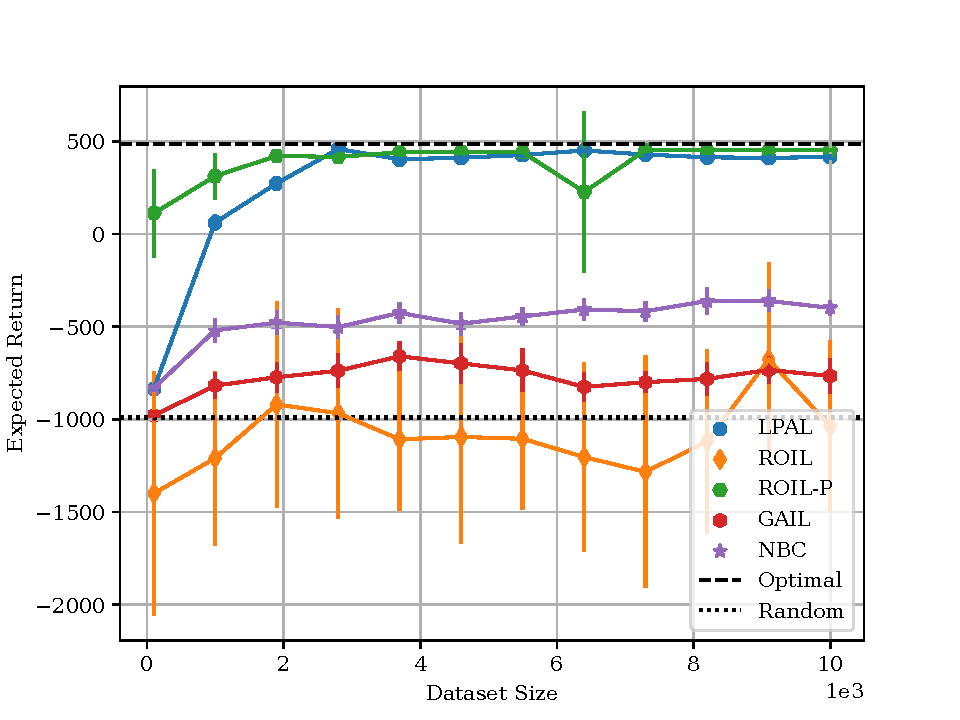
\includegraphics[width=0.45\textwidth]{figs/roil/40x40_driving_on_policy_returns.pdf}
	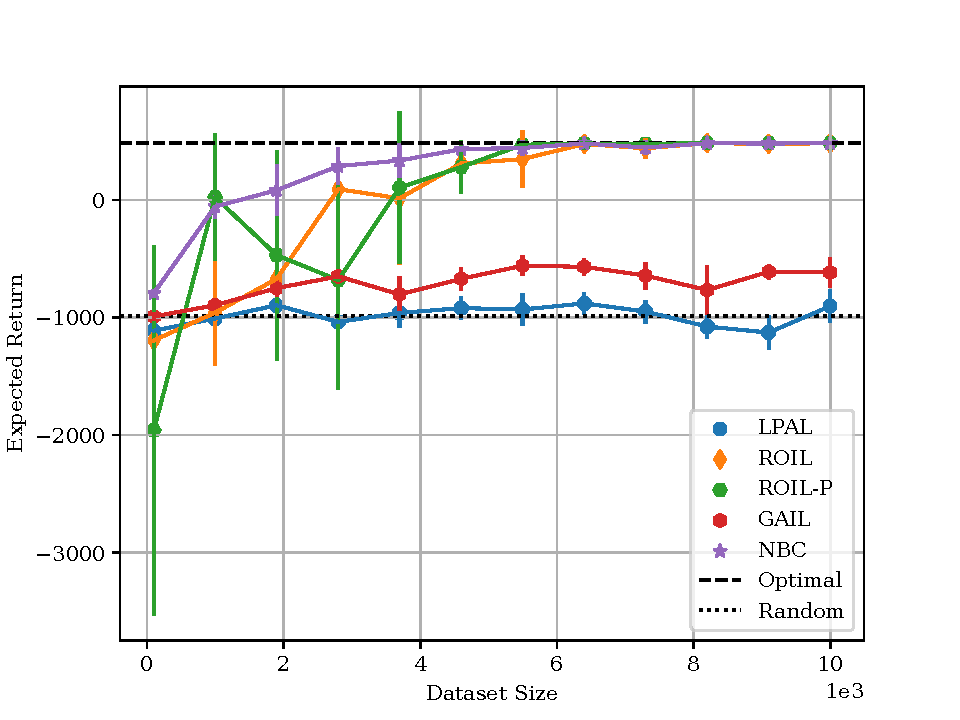
\includegraphics[width=0.45\textwidth]{figs/roil/40x40_driving_off_policy_returns.pdf}
	\caption{On (left) and off (right) policy 40x40 driving sim returns.}
	\label{fig:driving}
\end{figure}

\begin{figure}
	\centering
	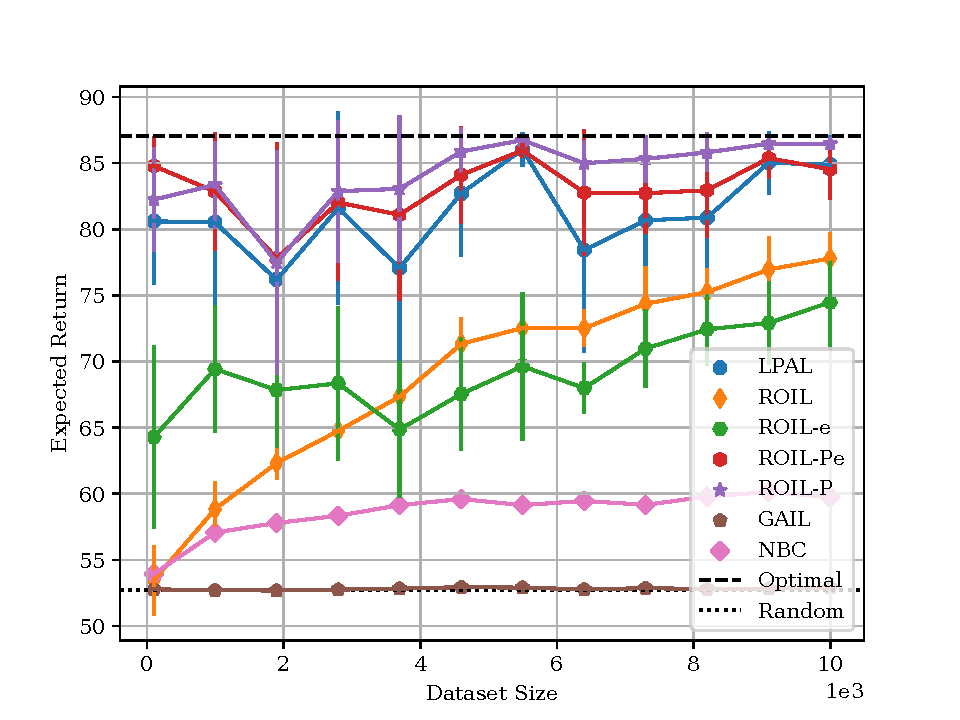
\includegraphics[width=0.45\textwidth]{figs/roil/40x40_gridworld_on_policy_all_returns.pdf}
	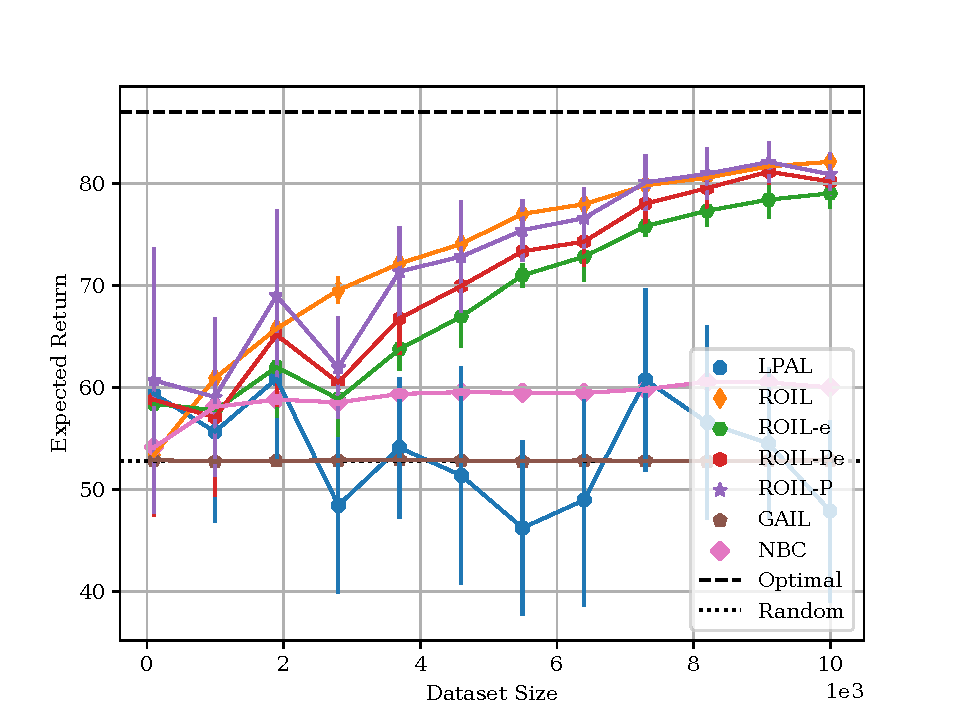
\includegraphics[width=0.45\textwidth]{figs/roil/40x40_gridworld_off_policy_all_returns.pdf}
	\caption{On (left) and off (right) policy 40x40 gridworld returns with more methods from \cref{sec:optimization-formulation}}
	\label{fig:more_methods_gridworld}
\end{figure}

\begin{figure}
	\centering
	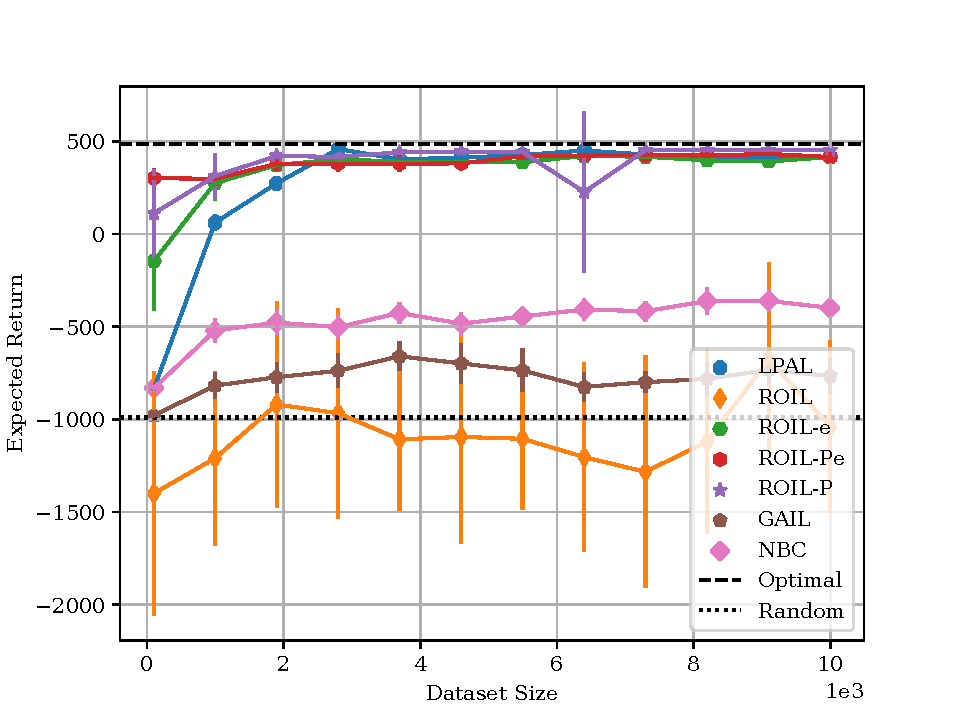
\includegraphics[width=0.45\textwidth]{figs/roil/40x40_driving_on_policy_all_returns.pdf}
	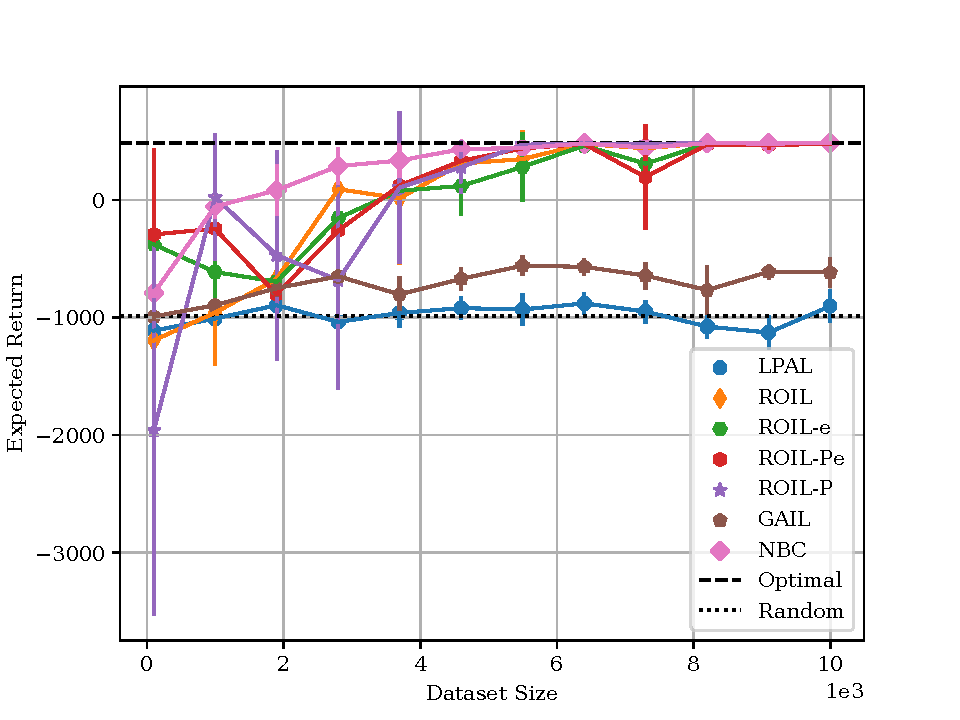
\includegraphics[width=0.45\textwidth]{figs/roil/40x40_driving_off_policy_all_returns.pdf}
	\caption{On (left) and off (right) policy 40x40 driving sim returns with more methods from \cref{sec:optimization-formulation}}
	\label{fig:more_methods_driving}
\end{figure}

We focus on describing the grid world environment; the driving environment is implemented similarly. The states of a grid world are integers from 0 to $N\times N$ where $N$ is the number of rows in the grid world, we assume we have square grid worlds where the number of columns and rows are the same. The actions an actor can take are up, down, left, and right. And the reward for a particular $(s,a)$ tuple is dictated by some reward vector $r \in \Real^{SA} = \Phi\tr w$ for some $w \in \mathcal{W}$. To solve all methods that rely on an LP, such as all ROIL variants described here, we rely on Gurobi~\cite{gurobi}. The feature vector for the grid world environment was the color of the current cell which was randomized for each seed, out of 4 total colors. For the driving simulator, there were also 4 features, current row, current column, whether the actor crashed in the current state, or whether the actor went off-road. \gersi{When constructing $D_e$ for off-policy experiments $\pi_e$ decides the actions for each state, however the state transitions came from a uniformly random policy $\pi_b$. More precisely $D_e = (s_t, \pi_e(s_t))_{t=0}^{D}$ where $s_{t+1} \sim P(s_t, \pi_b(s_t))$ and $s_0 \sim p_0$.}

\subsection{ROIL Variants}
\label{sec:roil_variants_appendix}
We focus on ROIL and ROIL-P. ROIL uses the linear constraint on $\mathcal{U}$ resulting in an outer minimization over $\Upsilon$ instead of $\mathcal{U}$ in \eqref{eq:extreme-points-reformulated} with the same inner maximization. ROIL-P uses pruning which is a technique to reduce the number of inner maximizations needed in the final minimization in \eqref{eq:extreme-points-reformulated}, we use $\hat{u}_e$ to prune away extreme points (or sampled points in cases where $\mathcal{W}$ leads to non-enumerable extreme points) where $\hat{u}_e\tr $ ext$(\mathcal{W}) \leq \tau$. 

For convenience, let $\psi \in \Real^d = \max_{v \in \Upsilon} v\tr\Phi w \;\; \forall w \in$ ext$(\mathcal{W})$ where $d$ is the number of inner maximizations you wish to solve, whether that be all extreme points of the L infinity norm ball or some sub-sample of a different norm ball. ROIL-P chooses $\tau$ to be the 90\% quantile of $\psi$. While it may seem ignorant to ignore some of these extreme points, it is a helpful heuristic that can help calibrate our pessimism as described in \cref{sec:optimization-formulation}. This extension as well as many others is what we find new and exciting about ROIL, however, we have too few pages to describe all such tweaks. For those interested, in \cref{fig:driving,fig:grid-40} we use $100$ samples from the $\Real_{1+}$ for ROIL-P.

We also implemented ROIL-e and ROIL-Pe which optimize over $\hat{\Upsilon}_\epsilon$ as in \cref{sec:incorp-addit-constr}, this led to comparable on policy performance to LPAL and ROIL-P while maintaining stable gains in expected return with new state action pairs off policy as seen in \cref{fig:more_methods_gridworld,fig:more_methods_driving}. However, due to how cluttered the graphs got, we decided to leave those as an extension and show off the two methods that were most representative of our formulation as a whole, putting the choice of robustness into the user's hands.

\subsection{GAIL}

While the performance of most methods seems about on par with what one would expect it may seem that our implementation of GAIL~\cite{Ho2016}
has some bugs. We assure the reader and refer the reader to our code \textcolor{red}{REDACTED} that we did indeed implement GAIL correctly and it does converge in smaller domains when $\mathcal{D}$ is on policy as the expectation in Algorithm 1 of~\cite{Ho2016} relies on $\hat{u}_{\mathrm{e}}$ being close to $u_{\mathrm{e}}\opt$. Due to computation constraints, and to be fair to the other methods we compared with, we had to limit the computation time per method. GAIL, being based on policy gradient methods, is rather sample inefficient concerning environment interactions~\cite[Section 7]{Ho2016} thus it incurs extra computation collecting on policy samples from $\pi_\theta$. We would also like to note that GAIL must bootstrap itself with a new random policy parameter $\theta$ each run as the other methods we tested against it also did not get to keep any information from previous runs.
% \roilLp*
% \begin{proof}
%   The result follows from the discussion in \cref{sec:basic-formulation} and by the epigraph formulation of~\eqref{eq:extreme-points-reformulated}.
    % Recall the definition of $\Phi \in \Real^{SA \times K}$ given some arbitrary ordering on $(s,a)$ pairs.
    % \begin{center}
    
    % 	\[\*\Phi\tr \;=\; \begin{bmatrix}
    % 			- & \phi_1\tr & - \\
    % 			- & \phi_2\tr & - \\
    % 			- & \vdots    & - \\
    % 			- & \phi_K\tr & -
    % 		\end{bmatrix}\]
    
    % 	Where $\phi_n = [\phi_n(s,a)\;\;\forall s,a \in S \times A]$ represents the n'th feature evaluated on each $(s,a)$ pair.
    % \end{center}
    
    % We apply a technique called Chebyshev Approximation~\cite{boyd_convex_optimization}(6.1) to equation~\eqref{eq:extreme_points_of_the_IRL_Formulation}.
    % This step can also be seen as writing~\eqref{eq:extreme_points_of_the_IRL_Formulation} in epigraph form.
    
    % \begin{equation}
    % 	\begin{mprog}
    % 		\minimize{u \in \mathcal{U}, \sigma \in \Real} \sigma
    % 		\stc \max_{v \in \Upsilon} |(v - u)\tr \Phi_i| \leq \sigma
    % 		\cs i \in 1 \dots k
    % 	\end{mprog}
    % \end{equation}
    
    % After expanding the absolute value is equivalent to.
    
    % \begin{equation}
    % 	\begin{mprog}
    % 		\minimize{u \in \mathcal{U}, \sigma \in \Real} \sigma
    % 		\stc \max_{v \in \Upsilon} (v - u)\tr \Phi_i \leq \sigma
    % 		\cs \max_{v \in \Upsilon} -(v - u)\tr \Phi_i \leq \sigma
    % 		\cs i \in 1 \dots k
    % 	\end{mprog}
    % \end{equation}
    
    % In order to make the above problem more easily solvable, let us take the dual of the first inner maximization problem.
    
    % \begin{equation}
    % 	\begin{mprog}
    % 		\maximize{v \in \Upsilon} (v - u)\tr \Phi_i
    % 		\cs i \in 1\dots k
    % 	\end{mprog}
    % \end{equation}
    
    % Notice in order to get this into an LP form we need to take the convex set $\Upsilon$ and construct a linear constraint which encapsulates what it means for an element $v \in \Real_+^{SA}$ to be in the set $\Upsilon$. Luckily this is easy to do as $\Upsilon$ is defined as a linear constraint on $\mathcal{U}$. For the sake of simplicity suppose that we consider one fixed $\Phi_i$, and omit the optimization over all $i \in 1\dots k$ for the duration
    % of the dual derivation. But do keep in mind, each feature vector gets its own dual variable.
    
    % \begin{equation}
    % 	\label{eq:primal_IRL_problem}
    % 	\begin{mprog}
    % 		\maximize{v \in \Real_+^{SA}} (v - u)\tr \Phi_i
    % 		\stc c\tr v = 0
    % 		\cs \sum_{a \in \mathcal{A}}(I - \gamma P_a\tr)v(\cdot, a) = p_0
    % 	\end{mprog}
    % \end{equation}
    
    % \begin{equation}
    % 	L(v, \alpha, \beta) = (v - u)\tr \Phi_i + \alpha c\tr v
    % 	+ \beta\tr (\sum_{a \in \mathcal{A}}(I - \gamma P_a\tr)v(\cdot, a) - p_0)
    % \end{equation}
    
    % Writing the summation as a matrix-vector multiplication we have.
    
    % \[\*A \;=\; \begin{bmatrix}
    % 		- & (I - \gamma P_1) & - \\
    % 		- & (I - \gamma P_2) & - \\
    % 		- & \vdots           & - \\
    % 		- & (I - \gamma P_a) & - \\
    % 	\end{bmatrix}\;\in\; \Real^{SA\times S}\]
    
    % \begin{equation}
    % 	\label{eq:rewrite_U_constraint}
    % 	L(v, \alpha, \beta) = (v - u)\tr \Phi_i + \alpha c\tr v
    % 	+ \beta\tr (A\tr v - p_0)
    % \end{equation}
    
    % Notice that we assume that the vector $v \in \Real^{SA}$ iterates over states first before iterating over actions.
    
    % \begin{equation}
    % 	g(\alpha, \beta) = \sup_{v\geq 0} L(v, \alpha, \beta)
    % \end{equation}
    
    % \begin{equation}
    % 	g(\alpha, \beta) = -u\tr \Phi_i - \beta\tr p_0 + \sup_{v\geq 0} (v\tr \Phi_i + \alpha c\tr v + \beta\tr A\tr v)
    % \end{equation}
    
    % \begin{equation}
    % 	g(\alpha, \beta) = -u\tr \Phi_i - \beta\tr p_0 + \sup_{v \geq 0} (\Phi_i\tr + \alpha c\tr + \beta\tr A\tr)v
    % \end{equation}
    
    % Notice that the quantity in the parentheses is linear in $v$, and linear functions are
    % bounded above if and only if their coefficient is 0.
    % Therefore, $g(\alpha, \beta) = \infty$ except for when $\Phi_i + \alpha c + A\beta \leq 0$ in which case
    % $g(\alpha, \beta) = -u\tr \Phi_i - \beta\tr p_0$.
    
    % Now we are ready to define the dual of~\eqref{eq:primal_IRL_problem}.
    % Given that $g(\alpha, \beta)$ is an upper bound on the optimal value of~\eqref{eq:primal_IRL_problem} for feasible $v$, we wish to minimize it.
    
    % \begin{equation}
    % 	\begin{mprog}
    % 		\minimize{\alpha \in \Real, \beta \in \Real^{S}} -u\tr \Phi_i - \beta\tr p_0
    % 		\stc \Phi_i + \alpha c + A\beta \leq 0
    % 	\end{mprog}
    % \end{equation}
    
    % Recall the formulation of the Chebyshev Center.
    % \begin{equation}
    % 	\begin{mprog}
    % 		\minimize{u \in \mathcal{U}, \sigma \in \Real} \sigma
    % 		\stc \max_{v \in \Upsilon} (v - u)\tr \Phi_i \leq \sigma
    % 		\cs \max_{v \in \Upsilon} -(v - u)\tr \Phi_i \leq \sigma
    % 		\cs i \in 1 \dots k
    % 	\end{mprog}
    % \end{equation}
    
    % Now derive a similar result for the second maximization using the same method as above and substitute.
    % Recall that each feature-vector has its own unique dual variables.
    
    % \begin{equation}
    % 	\begin{mprog}
    % 		\minimize{u\in\mathcal{U}, \sigma\in\Real} \sigma
    % 		\stc \min_{\alpha_i \in \Real, \beta_i \in \Real^{S}} -u\tr \Phi_i - \beta_i\tr p_0 \leq \sigma
    % 		\cs \Phi_i + \alpha_i c + A \beta_i \leq 0
    % 		\cs \min_{\hat{\alpha}_i \in \Real, \hat{\beta}_i \in \Real^{S}} u\tr \Phi_i - \hat{\beta}_i\tr p_0 \leq \sigma
    % 		\cs -\Phi_i + \hat{\alpha}_i c + A \hat{\beta}_i \leq 0
    % 		\cs i \in 1 \dots k
    % 	\end{mprog}
    % \end{equation}
    
    % \begin{equation}
    % 	\begin{mprog}
    % 		\label{eq:semi_fininished_LP}
    % 		\minimize{u\in\mathcal{U}, \sigma, \alpha_i, \hat{\alpha}_i \in \Real, \beta_i, \hat{\beta}_i \in \Real^{S}} \sigma
    % 		\stc -u\tr \Phi_i - \beta_i\tr p_0 \leq \sigma
    % 		\cs u\tr \Phi_i - \hat{\beta}_i\tr p_0 \leq \sigma
    % 		\cs \Phi_i + \alpha_i c + A \beta_i \leq 0
    % 		\cs -\Phi_i + \hat{\alpha}_i c + A \hat{\beta}_i \leq 0
    % 		\cs i \in 1 \dots k
    % 	\end{mprog}
    % \end{equation}
    
    % And now for the final push, notice that~\eqref{eq:semi_fininished_LP} is not an LP,
    % because of the nonlinear (yet convex) minimization over $u\in\mathcal{U}$. To remedy this notice
    % how we re-wrote the definition of $\mathcal{U}$ in~\eqref{eq:rewrite_U_constraint}. This leads us to the
    % LP formulation of the Chebyshev Center.
    % \gersi{TODO go back and explain why the $A^{T}v$ constraint makes sense}
    
    % \begin{equation}
    % 	\begin{mprog}
    % 		\minimize{\sigma, \alpha_i, \hat{\alpha}_i \in \Real, \beta_i, \hat{\beta}_i \in \Real^{S}, u \in \Real^{SA}} \sigma
    % 		\stc -u\tr \Phi_i - \beta_i\tr p_0 \leq \sigma
    % 		\cs u\tr \Phi_i - \hat{\beta}_i\tr p_0 \leq \sigma
    % 		\cs \Phi_i + \alpha_i c + A \beta_i \leq 0
    % 		\cs -\Phi_i + \hat{\alpha}_i c + A \hat{\beta}_i \leq 0
    % 		\cs i \in 1 \dots k
    % 		\cs A\tr u = p_0
    % 		\cs u \geq 0
    % 	\end{mprog}
    % \end{equation}
% \end{proof}


% \section{Proofs of \cref{sec:geom-intu-reduct} }

% \chebeyshevRegret*
% \begin{proof}
% 	For the sake of contradiction,
% 	assume there exists some $\pi' \in \Pi$ such that
% 	\[
% 		\max_{r\in \mathcal{R}} \max_{\pi \in \Pi_{R}(\mathcal{D})}
% 		\left(\rho(\pi,r) - \rho(\pi', r)\right) < \max_{r\in \mathcal{R}}
% 		\max_{\pi \in \Pi_{R}(\mathcal{D})}
% 		\left(\rho(\pi, r) - \rho(\hat{\pi}, r)\right)
% 	\]
% 	After algebraic manipulation, we have
% 	\begin{align*}
% 		\max_{r\in \mathcal{R}} \max_{\pi \in \Pi_{R}
% 			(\mathcal{D})} u_{\pi}\tr r - u_{\pi'}\tr r
% 		 & < \max_{r\in \mathcal{R}}
% 		\max_{\pi \in \Pi_{R}
% 			(\mathcal{D})} u_{\pi}\tr r - u_{\hat{\pi}}
% 		\tr r                                              \\
% 		\max_{r\in \mathcal{R}} \max_{\pi \in \Pi_{R}(\mathcal{D})}
% 		(u_{\pi} - u_{\pi'})\tr r
% 		 & < \max_{r\in \mathcal{R}}
% 		\max_{\pi \in \Pi_{R}(\mathcal{D})}
% 		(u_{\pi} - u_{\hat{\pi}})\tr r
% 		\\
% 		\max_{w\in \mathcal{W}} \max_{v \in \Upsilon} (v - u_{\pi'})\tr \Phi w
% 		 & < \max_{w\in \mathcal{W}} \max_{v \in \Upsilon}
% 		(v - u_{\hat{\pi}})\tr \Phi w
% 	\end{align*}
% 	Here, $u_{\pi}$, $u_{\pi'}$, and $u_{\hat{\pi}}$
% 	are the occupancy frequencies of their respective policies.

% 	Notice the change in the maximization objectives.
% 	We assume that $r = \Phi\tr w$ for some $w \in \mathcal{W}$,
% 	thus the maximization over $\mathcal{R}$ is equivalent to the maximization
% 	over $\mathcal{W}$ of $\Phi\tr w$.
% 	Secondly, by the occupancy frequency correspondence~\cite{Puterman1994}, the
% 	maximization over $\Pi_{\mathrm{R}}(\mathcal{D})$ is equivalent to the maximization over
% 	$\Upsilon$.
% 	Since $u_{\hat{\pi}} \in \arg\min_{u \in \mathcal{U}} \max_{w \in \mathcal{W}} \max_{v \in \Upsilon} {(v - u)}^T \Phi w$,
% 	this is a contradiction with the optimality of $\hat{\pi}$,
% 	therefore $\pi'$ cannot achieve less regret than $\hat{\pi}$.
% \end{proof}

% \paragraph{Relationship With LPAL, Syed and Schapire~\cite{Syed2008}}

% Theorem 5 of the LPAL paper~\cite{Syed2008} provides a bound on the performance of the policy returned by LPAL.
% In this section, we would like to provide insight into this bound using the notation of this paper.

% \begin{restatable}[LPAL bound]{theorem}{LPAL}
% \label{thm:LPAL}
% 	Let $\pi_{lp}$ be the policy returned by LPAL then
% 	\[V(\pi_{lp}) \geq V(\pi_{\mathrm{e}}) + v^* - 2\eps\]
% 	or equivalently expressed using occupancy frequencies
% 	\[u_{lp}\tr r \geq u_{\mathrm{e}}\tr r + v^* - 2\eps\]

% 	Where $\eps = \lvert\lvert \hat{u}_{\mathrm{e}}\tr \Phi - u_e\tr \Phi\rvert\rvert_*$
% \end{restatable}
% \begin{proof}
% 	Begin with the definitions
% 	\[
% 		u^* = \arg\min_{u \in \mathcal{U}} \lvert\lvert u\tr \Phi - \hat{u_{\mathrm{e}}}\tr \Phi \rvert\rvert_*
% 	\]
% 	\[
% 		v^* = - \lvert\lvert \Phi\tr u^* - \Phi\tr \hat{u_{\mathrm{e}}} \rvert\rvert_*
% 	\]
% 	Given that we wish to bound $V(\pi_{lp}) - V(\pi_{\mathrm{e}})$ lets begin with the definition of $V(\cdot)$.
% 	\[V(\pi_{lp}) - V(\pi_{\mathrm{e}}) = u_{lp}\tr r - u_e\tr r\]
% 	Both LPAL and our paper assumes that $r = \Phi\tr w$ for some $w \in \mathcal{W} = \Real_{1}$ LPAL calls the columns of $\Phi$ basis
% 	reward vectors, while we call them features but they are the same, save for notation.
% 	\[\geq \min_{w \in \mathcal{W}}(u_{lp}\tr \Phi w - u_{\mathrm{e}}\tr \Phi w) =- \max_{w \in \mathcal{W}}(u_e\tr \Phi - u_{lp}\tr \Phi)w \]
% 	Applying the definition of the dual norm with respect to $\mathcal{W}$
% 	\[= -\lvert\lvert u_{\mathrm{e}}\tr \Phi - u_{lp}\tr \Phi \rvert\rvert_*\]
% 	Now we apply the triangle inequality by adding 0
% 	\[= -\lvert\lvert u_{\mathrm{e}}\tr \Phi - \hat{u}_e + \hat{u}_e - u_{lp}\tr \Phi \rvert\rvert_*\]
% 	\[\geq -\lvert\lvert u_{\mathrm{e}}\tr \Phi - \hat{u}_e\rvert\rvert_* - \lvert\lvert \hat{u}_e - u_{lp}\tr \Phi \rvert\rvert_* = -\eps - \lvert\lvert \hat{u}_e - u_{lp}\tr \Phi \rvert\rvert_* \]
% 	\[\geq -\eps - \lvert\lvert \hat{u}_{\mathrm{e}}\tr \Phi - \Phi\tr u^*\rvert\rvert_*\]
% 	\[= -\eps - \lvert\lvert \hat{u}_{\mathrm{e}}\tr \Phi - u_e\tr\Phi + u_e\tr\Phi - \Phi\tr u^*\rvert\rvert_*\]
% 	\[\geq -\eps - \lvert\lvert \hat{u}_{\mathrm{e}}\tr \Phi - u_e\tr\Phi\rvert\rvert_* - \lvert\lvert u_e\tr\Phi - \Phi\tr u^*\rvert\rvert_*\]
% 	\[= -2\eps - \lvert\lvert u_{\mathrm{e}}\tr\Phi - \Phi\tr u^*\rvert\rvert_* = -2\eps + v^*\]
% \end{proof}
